\documentclass[ignorenonframetext,]{beamer}
\setbeamertemplate{caption}[numbered]
\setbeamertemplate{caption label separator}{: }
\setbeamercolor{caption name}{fg=normal text.fg}
\beamertemplatenavigationsymbolsempty
\usepackage{lmodern}
\usepackage{amssymb,amsmath}
\usepackage{ifxetex,ifluatex}
\usepackage{fixltx2e} % provides \textsubscript
\ifnum 0\ifxetex 1\fi\ifluatex 1\fi=0 % if pdftex
  \usepackage[T1]{fontenc}
  \usepackage[utf8]{inputenc}
\else % if luatex or xelatex
  \ifxetex
    \usepackage{mathspec}
  \else
    \usepackage{fontspec}
  \fi
  \defaultfontfeatures{Ligatures=TeX,Scale=MatchLowercase}
\fi
\usetheme[]{CambridgeUS}
\usecolortheme{beaver}
\usefonttheme{structurebold}
% use upquote if available, for straight quotes in verbatim environments
\IfFileExists{upquote.sty}{\usepackage{upquote}}{}
% use microtype if available
\IfFileExists{microtype.sty}{%
\usepackage{microtype}
\UseMicrotypeSet[protrusion]{basicmath} % disable protrusion for tt fonts
}{}
\newif\ifbibliography
\hypersetup{
            pdftitle={B3 - Linear Regression},
            pdfauthor={Jan-Philipp Kolb},
            pdfborder={0 0 0},
            breaklinks=true}
\urlstyle{same}  % don't use monospace font for urls
\usepackage{color}
\usepackage{fancyvrb}
\newcommand{\VerbBar}{|}
\newcommand{\VERB}{\Verb[commandchars=\\\{\}]}
\DefineVerbatimEnvironment{Highlighting}{Verbatim}{commandchars=\\\{\}}
% Add ',fontsize=\small' for more characters per line
\usepackage{framed}
\definecolor{shadecolor}{RGB}{248,248,248}
\newenvironment{Shaded}{\begin{snugshade}}{\end{snugshade}}
\newcommand{\KeywordTok}[1]{\textcolor[rgb]{0.13,0.29,0.53}{\textbf{#1}}}
\newcommand{\DataTypeTok}[1]{\textcolor[rgb]{0.13,0.29,0.53}{#1}}
\newcommand{\DecValTok}[1]{\textcolor[rgb]{0.00,0.00,0.81}{#1}}
\newcommand{\BaseNTok}[1]{\textcolor[rgb]{0.00,0.00,0.81}{#1}}
\newcommand{\FloatTok}[1]{\textcolor[rgb]{0.00,0.00,0.81}{#1}}
\newcommand{\ConstantTok}[1]{\textcolor[rgb]{0.00,0.00,0.00}{#1}}
\newcommand{\CharTok}[1]{\textcolor[rgb]{0.31,0.60,0.02}{#1}}
\newcommand{\SpecialCharTok}[1]{\textcolor[rgb]{0.00,0.00,0.00}{#1}}
\newcommand{\StringTok}[1]{\textcolor[rgb]{0.31,0.60,0.02}{#1}}
\newcommand{\VerbatimStringTok}[1]{\textcolor[rgb]{0.31,0.60,0.02}{#1}}
\newcommand{\SpecialStringTok}[1]{\textcolor[rgb]{0.31,0.60,0.02}{#1}}
\newcommand{\ImportTok}[1]{#1}
\newcommand{\CommentTok}[1]{\textcolor[rgb]{0.56,0.35,0.01}{\textit{#1}}}
\newcommand{\DocumentationTok}[1]{\textcolor[rgb]{0.56,0.35,0.01}{\textbf{\textit{#1}}}}
\newcommand{\AnnotationTok}[1]{\textcolor[rgb]{0.56,0.35,0.01}{\textbf{\textit{#1}}}}
\newcommand{\CommentVarTok}[1]{\textcolor[rgb]{0.56,0.35,0.01}{\textbf{\textit{#1}}}}
\newcommand{\OtherTok}[1]{\textcolor[rgb]{0.56,0.35,0.01}{#1}}
\newcommand{\FunctionTok}[1]{\textcolor[rgb]{0.00,0.00,0.00}{#1}}
\newcommand{\VariableTok}[1]{\textcolor[rgb]{0.00,0.00,0.00}{#1}}
\newcommand{\ControlFlowTok}[1]{\textcolor[rgb]{0.13,0.29,0.53}{\textbf{#1}}}
\newcommand{\OperatorTok}[1]{\textcolor[rgb]{0.81,0.36,0.00}{\textbf{#1}}}
\newcommand{\BuiltInTok}[1]{#1}
\newcommand{\ExtensionTok}[1]{#1}
\newcommand{\PreprocessorTok}[1]{\textcolor[rgb]{0.56,0.35,0.01}{\textit{#1}}}
\newcommand{\AttributeTok}[1]{\textcolor[rgb]{0.77,0.63,0.00}{#1}}
\newcommand{\RegionMarkerTok}[1]{#1}
\newcommand{\InformationTok}[1]{\textcolor[rgb]{0.56,0.35,0.01}{\textbf{\textit{#1}}}}
\newcommand{\WarningTok}[1]{\textcolor[rgb]{0.56,0.35,0.01}{\textbf{\textit{#1}}}}
\newcommand{\AlertTok}[1]{\textcolor[rgb]{0.94,0.16,0.16}{#1}}
\newcommand{\ErrorTok}[1]{\textcolor[rgb]{0.64,0.00,0.00}{\textbf{#1}}}
\newcommand{\NormalTok}[1]{#1}
\usepackage{longtable,booktabs}
\usepackage{caption}
% These lines are needed to make table captions work with longtable:
\makeatletter
\def\fnum@table{\tablename~\thetable}
\makeatother
\usepackage{graphicx,grffile}
\makeatletter
\def\maxwidth{\ifdim\Gin@nat@width>\linewidth\linewidth\else\Gin@nat@width\fi}
\def\maxheight{\ifdim\Gin@nat@height>\textheight0.8\textheight\else\Gin@nat@height\fi}
\makeatother
% Scale images if necessary, so that they will not overflow the page
% margins by default, and it is still possible to overwrite the defaults
% using explicit options in \includegraphics[width, height, ...]{}
\setkeys{Gin}{width=\maxwidth,height=\maxheight,keepaspectratio}

% Prevent slide breaks in the middle of a paragraph:
\widowpenalties 1 10000
\raggedbottom

\AtBeginPart{
  \let\insertpartnumber\relax
  \let\partname\relax
  \frame{\partpage}
}
\AtBeginSection{
  \ifbibliography
  \else
    \let\insertsectionnumber\relax
    \let\sectionname\relax
    \frame{\sectionpage}
  \fi
}
\AtBeginSubsection{
  \let\insertsubsectionnumber\relax
  \let\subsectionname\relax
  \frame{\subsectionpage}
}

\setlength{\parindent}{0pt}
\setlength{\parskip}{6pt plus 2pt minus 1pt}
\setlength{\emergencystretch}{3em}  % prevent overfull lines
\providecommand{\tightlist}{%
  \setlength{\itemsep}{0pt}\setlength{\parskip}{0pt}}
\setcounter{secnumdepth}{0}

\title{B3 - Linear Regression}
\author{Jan-Philipp Kolb}
\date{16 Oktober 2018}

\begin{document}
\frame{\titlepage}

\begin{frame}{Gute Literatur für lineare Regression in R}

\begin{block}{J H Maindonald -
\href{https://cran.r-project.org/doc/contrib/usingR.pdf}{Using R for
Data Analysis and Graphics Introduction, Code and Commentary}}

\begin{itemize}
\tightlist
\item
  Introduction to R
\item
  Data analysis
\item
  Statistical models
\item
  Inference concepts
\item
  Regression with one predictor
\item
  Multiple linear regression
\item
  Extending the linear model
\item
  \ldots{}
\end{itemize}

\end{block}

\end{frame}

\begin{frame}[fragile]{Variablen im \texttt{mtcars} Datensatz}

Hilfe File für den \texttt{roller} Datensatz:

\begin{Shaded}
\begin{Highlighting}[]
\NormalTok{?mtcars}
\end{Highlighting}
\end{Shaded}

\begin{itemize}
\tightlist
\item
  mpg - Meilen/(US) Gallone
\item
  cyl - Anzahl der Zylinder
\end{itemize}

\end{frame}

\begin{frame}{Datensatz \texttt{mtcars}}

\begin{longtable}[]{@{}lrrrrrrrrrrr@{}}
\toprule
& mpg & cyl & disp & hp & drat & wt & qsec & vs & am & gear &
carb\tabularnewline
\midrule
\endhead
Mazda RX4 & 21.0 & 6 & 160.0 & 110 & 3.90 & 2.620 & 16.46 & 0 & 1 & 4 &
4\tabularnewline
Mazda RX4 Wag & 21.0 & 6 & 160.0 & 110 & 3.90 & 2.875 & 17.02 & 0 & 1 &
4 & 4\tabularnewline
Datsun 710 & 22.8 & 4 & 108.0 & 93 & 3.85 & 2.320 & 18.61 & 1 & 1 & 4 &
1\tabularnewline
Hornet 4 Drive & 21.4 & 6 & 258.0 & 110 & 3.08 & 3.215 & 19.44 & 1 & 0 &
3 & 1\tabularnewline
Hornet Sportabout & 18.7 & 8 & 360.0 & 175 & 3.15 & 3.440 & 17.02 & 0 &
0 & 3 & 2\tabularnewline
Valiant & 18.1 & 6 & 225.0 & 105 & 2.76 & 3.460 & 20.22 & 1 & 0 & 3 &
1\tabularnewline
Duster 360 & 14.3 & 8 & 360.0 & 245 & 3.21 & 3.570 & 15.84 & 0 & 0 & 3 &
4\tabularnewline
Merc 240D & 24.4 & 4 & 146.7 & 62 & 3.69 & 3.190 & 20.00 & 1 & 0 & 4 &
2\tabularnewline
Merc 230 & 22.8 & 4 & 140.8 & 95 & 3.92 & 3.150 & 22.90 & 1 & 0 & 4 &
2\tabularnewline
Merc 280 & 19.2 & 6 & 167.6 & 123 & 3.92 & 3.440 & 18.30 & 1 & 0 & 4 &
4\tabularnewline
Merc 280C & 17.8 & 6 & 167.6 & 123 & 3.92 & 3.440 & 18.90 & 1 & 0 & 4 &
4\tabularnewline
Merc 450SE & 16.4 & 8 & 275.8 & 180 & 3.07 & 4.070 & 17.40 & 0 & 0 & 3 &
3\tabularnewline
Merc 450SL & 17.3 & 8 & 275.8 & 180 & 3.07 & 3.730 & 17.60 & 0 & 0 & 3 &
3\tabularnewline
Merc 450SLC & 15.2 & 8 & 275.8 & 180 & 3.07 & 3.780 & 18.00 & 0 & 0 & 3
& 3\tabularnewline
Cadillac Fleetwood & 10.4 & 8 & 472.0 & 205 & 2.93 & 5.250 & 17.98 & 0 &
0 & 3 & 4\tabularnewline
Lincoln Continental & 10.4 & 8 & 460.0 & 215 & 3.00 & 5.424 & 17.82 & 0
& 0 & 3 & 4\tabularnewline
Chrysler Imperial & 14.7 & 8 & 440.0 & 230 & 3.23 & 5.345 & 17.42 & 0 &
0 & 3 & 4\tabularnewline
Fiat 128 & 32.4 & 4 & 78.7 & 66 & 4.08 & 2.200 & 19.47 & 1 & 1 & 4 &
1\tabularnewline
Honda Civic & 30.4 & 4 & 75.7 & 52 & 4.93 & 1.615 & 18.52 & 1 & 1 & 4 &
2\tabularnewline
Toyota Corolla & 33.9 & 4 & 71.1 & 65 & 4.22 & 1.835 & 19.90 & 1 & 1 & 4
& 1\tabularnewline
Toyota Corona & 21.5 & 4 & 120.1 & 97 & 3.70 & 2.465 & 20.01 & 1 & 0 & 3
& 1\tabularnewline
Dodge Challenger & 15.5 & 8 & 318.0 & 150 & 2.76 & 3.520 & 16.87 & 0 & 0
& 3 & 2\tabularnewline
AMC Javelin & 15.2 & 8 & 304.0 & 150 & 3.15 & 3.435 & 17.30 & 0 & 0 & 3
& 2\tabularnewline
Camaro Z28 & 13.3 & 8 & 350.0 & 245 & 3.73 & 3.840 & 15.41 & 0 & 0 & 3 &
4\tabularnewline
Pontiac Firebird & 19.2 & 8 & 400.0 & 175 & 3.08 & 3.845 & 17.05 & 0 & 0
& 3 & 2\tabularnewline
Fiat X1-9 & 27.3 & 4 & 79.0 & 66 & 4.08 & 1.935 & 18.90 & 1 & 1 & 4 &
1\tabularnewline
Porsche 914-2 & 26.0 & 4 & 120.3 & 91 & 4.43 & 2.140 & 16.70 & 0 & 1 & 5
& 2\tabularnewline
Lotus Europa & 30.4 & 4 & 95.1 & 113 & 3.77 & 1.513 & 16.90 & 1 & 1 & 5
& 2\tabularnewline
Ford Pantera L & 15.8 & 8 & 351.0 & 264 & 4.22 & 3.170 & 14.50 & 0 & 1 &
5 & 4\tabularnewline
Ferrari Dino & 19.7 & 6 & 145.0 & 175 & 3.62 & 2.770 & 15.50 & 0 & 1 & 5
& 6\tabularnewline
Maserati Bora & 15.0 & 8 & 301.0 & 335 & 3.54 & 3.570 & 14.60 & 0 & 1 &
5 & 8\tabularnewline
Volvo 142E & 21.4 & 4 & 121.0 & 109 & 4.11 & 2.780 & 18.60 & 1 & 1 & 4 &
2\tabularnewline
\bottomrule
\end{longtable}

\end{frame}

\begin{frame}[fragile]{Verteilungen von zwei Variablen aus dem Datensatz
\texttt{mtcars}}

\begin{Shaded}
\begin{Highlighting}[]
\KeywordTok{par}\NormalTok{(}\DataTypeTok{mfrow=}\KeywordTok{c}\NormalTok{(}\DecValTok{1}\NormalTok{,}\DecValTok{2}\NormalTok{))}
\KeywordTok{plot}\NormalTok{(}\KeywordTok{density}\NormalTok{(mtcars}\OperatorTok{$}\NormalTok{wt)); }\KeywordTok{plot}\NormalTok{(}\KeywordTok{density}\NormalTok{(mtcars}\OperatorTok{$}\NormalTok{mpg))}
\end{Highlighting}
\end{Shaded}

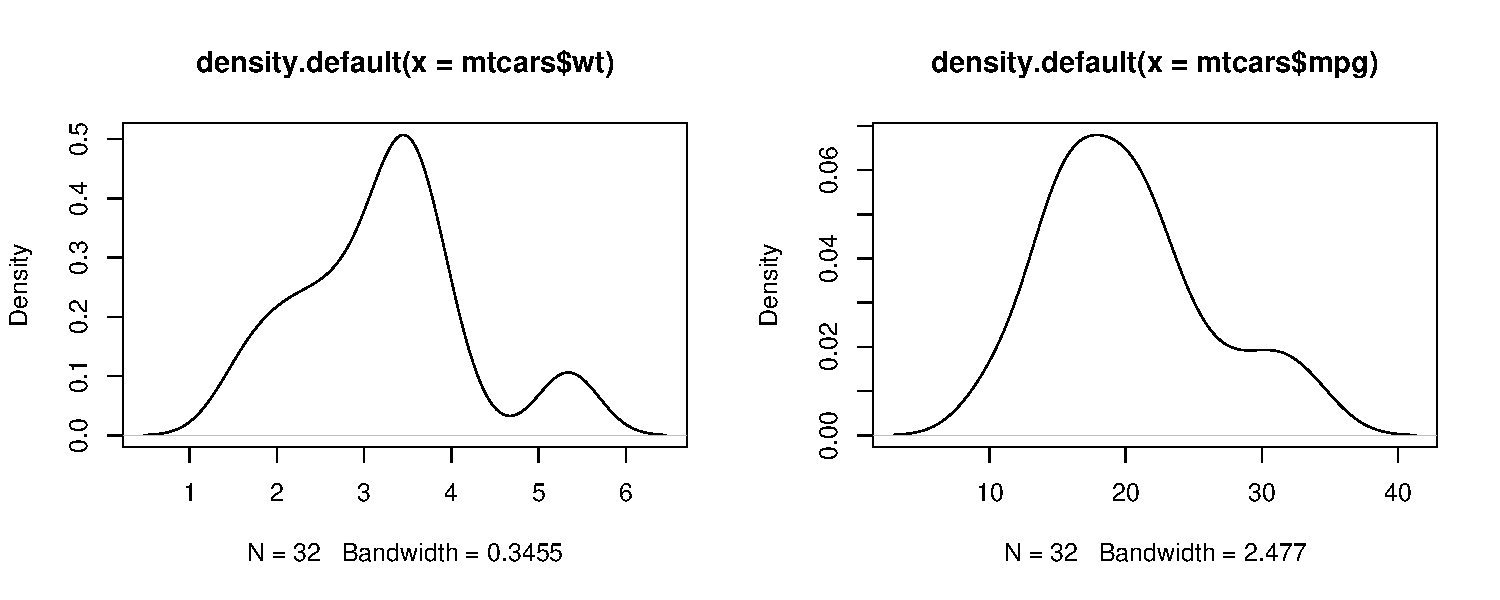
\includegraphics{B3_linreg_files/figure-beamer/unnamed-chunk-5-1.pdf}

\end{frame}

\begin{frame}[fragile]{Ein einfaches Regressionsmodell}

\begin{block}{Abhängige Variable - Meilen pro Gallone (\texttt{mpg})}

\end{block}

\begin{block}{Unabhängige Variable - Gewicht (\texttt{wt})}

\begin{Shaded}
\begin{Highlighting}[]
\NormalTok{m1 <-}\StringTok{ }\KeywordTok{lm}\NormalTok{(mpg }\OperatorTok{~}\StringTok{ }\NormalTok{wt,}\DataTypeTok{data=}\NormalTok{mtcars)}
\NormalTok{m1}
\end{Highlighting}
\end{Shaded}

\begin{verbatim}
## 
## Call:
## lm(formula = mpg ~ wt, data = mtcars)
## 
## Coefficients:
## (Intercept)           wt  
##      37.285       -5.344
\end{verbatim}

\end{block}

\end{frame}

\begin{frame}[fragile]{Die Modell Zusammenfassung:}

\begin{Shaded}
\begin{Highlighting}[]
\KeywordTok{summary}\NormalTok{(m1) }
\end{Highlighting}
\end{Shaded}

\begin{verbatim}
## 
## Call:
## lm(formula = mpg ~ wt, data = mtcars)
## 
## Residuals:
##     Min      1Q  Median      3Q     Max 
## -4.5432 -2.3647 -0.1252  1.4096  6.8727 
## 
## Coefficients:
##             Estimate Std. Error t value Pr(>|t|)    
## (Intercept)  37.2851     1.8776  19.858  < 2e-16 ***
## wt           -5.3445     0.5591  -9.559 1.29e-10 ***
## ---
## Signif. codes:  0 '***' 0.001 '**' 0.01 '*' 0.05 '.' 0.1 ' ' 1
## 
## Residual standard error: 3.046 on 30 degrees of freedom
## Multiple R-squared:  0.7528, Adjusted R-squared:  0.7446 
## F-statistic: 91.38 on 1 and 30 DF,  p-value: 1.294e-10
\end{verbatim}

\end{frame}

\begin{frame}[fragile]{Die Modellformel}

\begin{block}{Modell ohne Achsenabschnitt}

\begin{Shaded}
\begin{Highlighting}[]
\NormalTok{m2 <-}\StringTok{ }\KeywordTok{lm}\NormalTok{(mpg }\OperatorTok{~}\StringTok{ }\OperatorTok{-}\StringTok{ }\DecValTok{1} \OperatorTok{+}\StringTok{ }\NormalTok{wt,}\DataTypeTok{data=}\NormalTok{mtcars)}
\KeywordTok{summary}\NormalTok{(m2)}\OperatorTok{$}\NormalTok{coefficients}
\end{Highlighting}
\end{Shaded}

\begin{verbatim}
##    Estimate Std. Error  t value    Pr(>|t|)
## wt 5.291624  0.5931801 8.920771 4.55314e-10
\end{verbatim}

\end{block}

\begin{block}{Weitere Variablen hinzufügen}

\begin{Shaded}
\begin{Highlighting}[]
\NormalTok{m3 <-}\StringTok{ }\KeywordTok{lm}\NormalTok{(mpg }\OperatorTok{~}\StringTok{ }\NormalTok{wt }\OperatorTok{+}\StringTok{ }\NormalTok{cyl,}\DataTypeTok{data=}\NormalTok{mtcars)}
\KeywordTok{summary}\NormalTok{(m3)}\OperatorTok{$}\NormalTok{coefficients}
\end{Highlighting}
\end{Shaded}

\begin{verbatim}
##              Estimate Std. Error   t value     Pr(>|t|)
## (Intercept) 39.686261  1.7149840 23.140893 3.043182e-20
## wt          -3.190972  0.7569065 -4.215808 2.220200e-04
## cyl         -1.507795  0.4146883 -3.635972 1.064282e-03
\end{verbatim}

\end{block}

\end{frame}

\begin{frame}[fragile]{\href{https://cran.r-project.org/web/packages/Formula/vignettes/Formula.pdf}{\textbf{Weitere
Möglichkeiten, die Formel zu spezifizieren}}}

\begin{block}{Interaktionseffekt}

\begin{Shaded}
\begin{Highlighting}[]
\CommentTok{# effect of cyl and interaction effect:}
\NormalTok{m3a<-}\KeywordTok{lm}\NormalTok{(mpg}\OperatorTok{~}\NormalTok{wt}\OperatorTok{*}\NormalTok{cyl,}\DataTypeTok{data=}\NormalTok{mtcars) }

\CommentTok{# only interaction effect:}
\NormalTok{m3b<-}\KeywordTok{lm}\NormalTok{(mpg}\OperatorTok{~}\NormalTok{wt}\OperatorTok{:}\NormalTok{cyl,}\DataTypeTok{data=}\NormalTok{mtcars) }
\end{Highlighting}
\end{Shaded}

\end{block}

\begin{block}{Den Logarithmus nehmen}

\begin{Shaded}
\begin{Highlighting}[]
\NormalTok{m3d<-}\KeywordTok{lm}\NormalTok{(mpg}\OperatorTok{~}\KeywordTok{log}\NormalTok{(wt),}\DataTypeTok{data=}\NormalTok{mtcars) }
\end{Highlighting}
\end{Shaded}

\end{block}

\end{frame}

\begin{frame}[fragile]{Ein Modell mit Interaktionseffekt}

\begin{block}{Variable \texttt{disp} - Hubraum}

\begin{Shaded}
\begin{Highlighting}[]
\NormalTok{m3d<-}\KeywordTok{lm}\NormalTok{(mpg}\OperatorTok{~}\NormalTok{wt}\OperatorTok{*}\NormalTok{disp,}\DataTypeTok{data=}\NormalTok{mtcars) }
\NormalTok{m3dsum <-}\StringTok{ }\KeywordTok{summary}\NormalTok{(m3d)}
\NormalTok{m3dsum}\OperatorTok{$}\NormalTok{coefficients}
\end{Highlighting}
\end{Shaded}

\begin{verbatim}
##                Estimate  Std. Error   t value     Pr(>|t|)
## (Intercept) 44.08199770 3.123062627 14.114990 2.955567e-14
## wt          -6.49567966 1.313382622 -4.945763 3.216705e-05
## disp        -0.05635816 0.013238696 -4.257078 2.101721e-04
## wt:disp      0.01170542 0.003255102  3.596022 1.226988e-03
\end{verbatim}

\end{block}

\end{frame}

\begin{frame}[fragile]{\href{https://cran.r-project.org/web/packages/jtools/vignettes/interactions.html}{\textbf{Interaktionen
untersuchen}}}

\begin{block}{\texttt{jtools} - Analysis and Presentation of Social
Scientific Data}

\begin{Shaded}
\begin{Highlighting}[]
\KeywordTok{library}\NormalTok{(jtools)}
\KeywordTok{interact_plot}\NormalTok{(m3d, }\DataTypeTok{pred =} \StringTok{"wt"}\NormalTok{, }\DataTypeTok{modx =} \StringTok{"disp"}\NormalTok{)}
\end{Highlighting}
\end{Shaded}

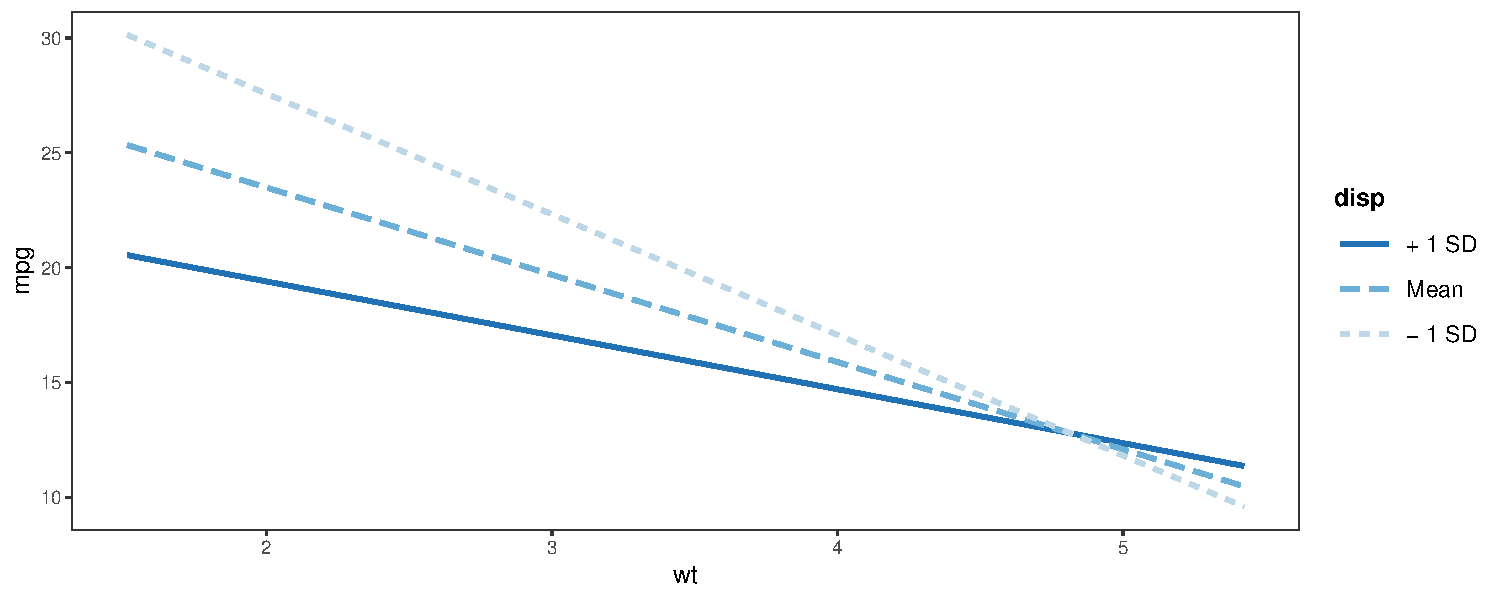
\includegraphics{B3_linreg_files/figure-beamer/unnamed-chunk-15-1.pdf}

\begin{itemize}
\tightlist
\item
  Wenn Interaktions-Variable stetig (hier \texttt{disp}) erhält man drei
  Linien:
\item
  1 - (mw), 2 - (mw - sd) und (mw + sd)
\end{itemize}

\end{block}

\end{frame}

\begin{frame}[fragile]{Das R-Paket \texttt{interplot}}

\begin{quote}
Plot the Effects of Variables in Interaction Terms
\end{quote}

\begin{Shaded}
\begin{Highlighting}[]
\KeywordTok{library}\NormalTok{(interplot)}
\end{Highlighting}
\end{Shaded}

\begin{itemize}
\tightlist
\item
  Eine detailliertere Erklärung findet man in der
  \href{https://cran.r-project.org/web/packages/interplot/vignettes/interplot-vignette.html}{\textbf{\texttt{Interplot}}}
  Vignette
\end{itemize}


\includegraphics{figure/interplot_vignette.PNG}

\end{frame}

\begin{frame}[fragile]{Das R-Paket \texttt{interplot}}

\begin{itemize}
\tightlist
\item
  Der Effekt wird auf der y Achse abgetragen - \texttt{wt} auf der
  x-Achse
\end{itemize}

\begin{Shaded}
\begin{Highlighting}[]
\KeywordTok{interplot}\NormalTok{(}\DataTypeTok{m =}\NormalTok{ m3a, }\DataTypeTok{var1 =} \StringTok{"wt"}\NormalTok{, }\DataTypeTok{var2 =} \StringTok{"cyl"}\NormalTok{, }\DataTypeTok{hist =} \OtherTok{TRUE}\NormalTok{)  }
\end{Highlighting}
\end{Shaded}

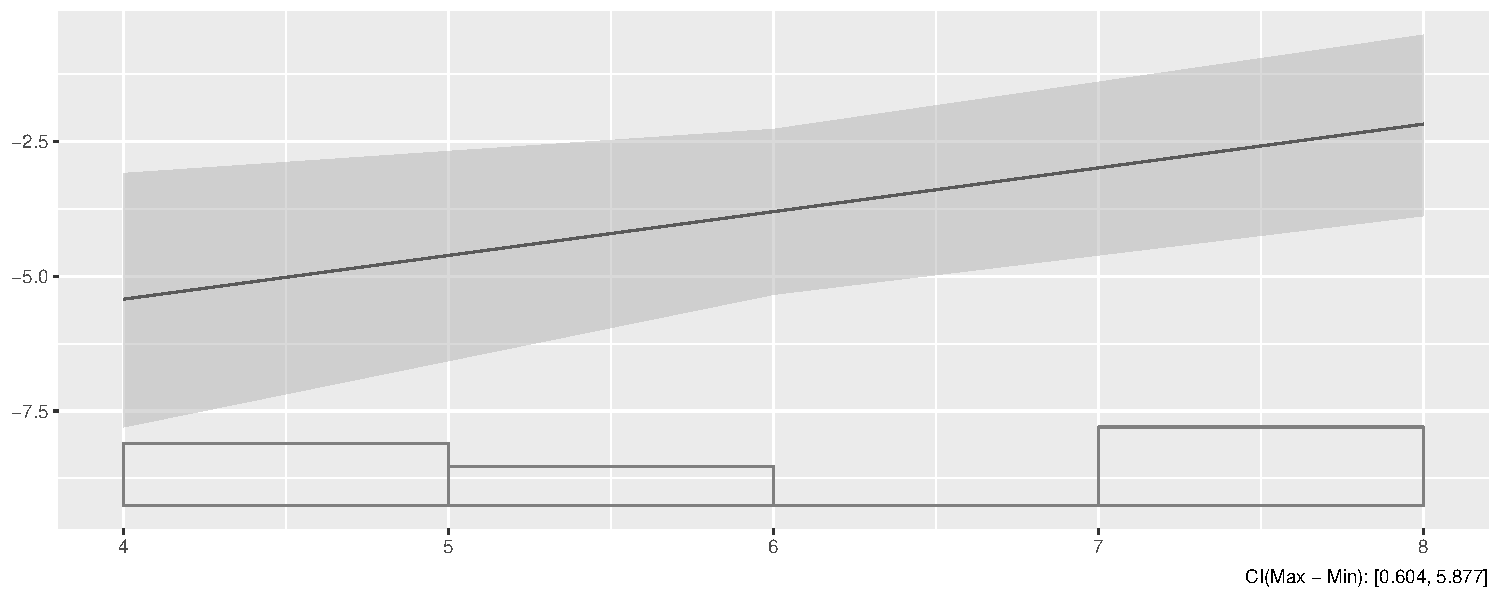
\includegraphics{B3_linreg_files/figure-beamer/unnamed-chunk-19-1.pdf}

\end{frame}

\begin{frame}[fragile]{Beispiel: Objekt Orientierung}

\begin{itemize}
\tightlist
\item
  \texttt{m3} ist nun ein spezielles Regressionsobjekt
\item
  Verschiedene Funktionen können auf dieses Objekt angewendet werden.
\end{itemize}

\begin{Shaded}
\begin{Highlighting}[]
\KeywordTok{predict}\NormalTok{(m3) }\CommentTok{# Prediction}
\KeywordTok{resid}\NormalTok{(m3) }\CommentTok{# Residuals}
\end{Highlighting}
\end{Shaded}

\begin{verbatim}
##         Mazda RX4     Mazda RX4 Wag        Datsun 710    Hornet 4 Drive 
##          22.27914          21.46545          26.25203          20.38052 
## Hornet Sportabout           Valiant 
##          16.64696          19.59873
\end{verbatim}

\begin{verbatim}
##         Mazda RX4     Mazda RX4 Wag        Datsun 710    Hornet 4 Drive 
##        -1.2791447        -0.4654468        -3.4520262         1.0194838 
## Hornet Sportabout           Valiant 
##         2.0530424        -1.4987281
\end{verbatim}

\end{frame}

\begin{frame}[fragile]{Eine Modellvorhersage machen}

\begin{Shaded}
\begin{Highlighting}[]
\NormalTok{pre <-}\StringTok{ }\KeywordTok{predict}\NormalTok{(m1)}
\KeywordTok{head}\NormalTok{(mtcars}\OperatorTok{$}\NormalTok{mpg)}
\end{Highlighting}
\end{Shaded}

\begin{verbatim}
## [1] 21.0 21.0 22.8 21.4 18.7 18.1
\end{verbatim}

\begin{Shaded}
\begin{Highlighting}[]
\KeywordTok{head}\NormalTok{(pre)}
\end{Highlighting}
\end{Shaded}

\begin{verbatim}
##         Mazda RX4     Mazda RX4 Wag        Datsun 710    Hornet 4 Drive 
##          23.28261          21.91977          24.88595          20.10265 
## Hornet Sportabout           Valiant 
##          18.90014          18.79325
\end{verbatim}

\end{frame}

\begin{frame}[fragile]{Residuenplot - Modellannahmen verletzt?}

\begin{itemize}
\tightlist
\item
  Gibt es ein Muster in der Abweichung von der Linie
\end{itemize}

\begin{Shaded}
\begin{Highlighting}[]
\KeywordTok{plot}\NormalTok{(m3,}\DecValTok{1}\NormalTok{)}
\end{Highlighting}
\end{Shaded}

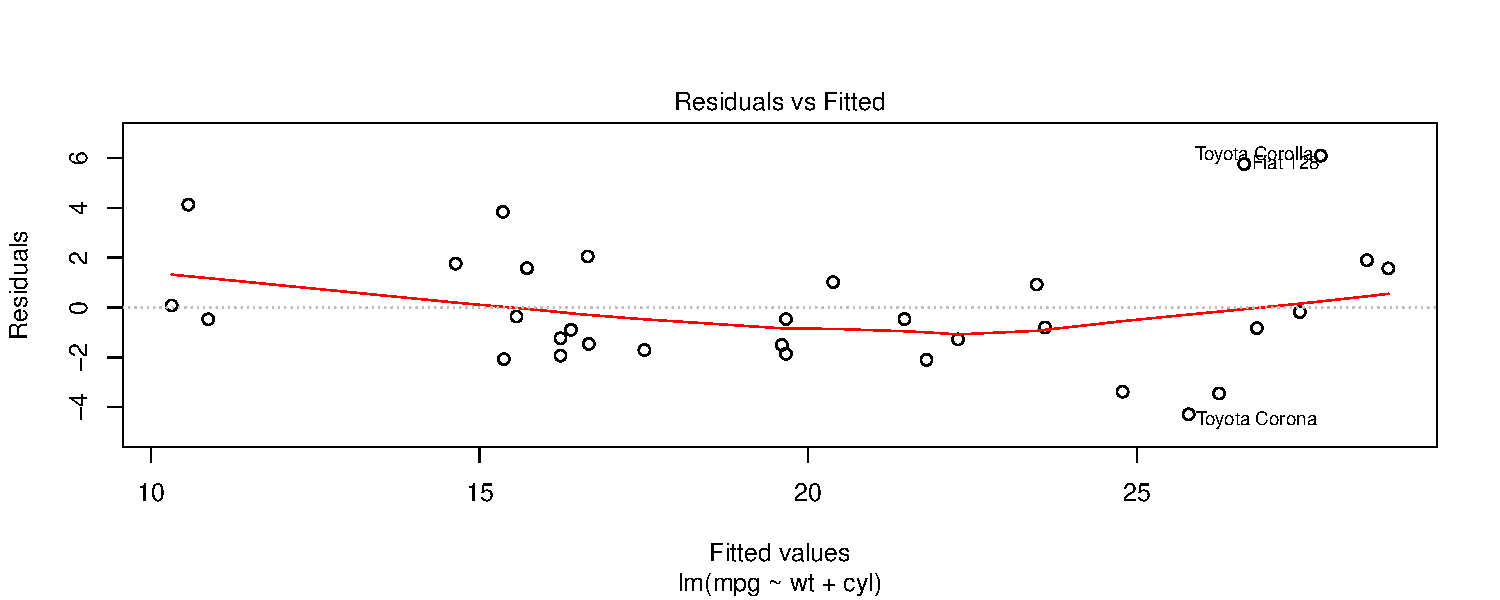
\includegraphics{B3_linreg_files/figure-beamer/unnamed-chunk-23-1.pdf}

\end{frame}

\begin{frame}[fragile]{Residuenplot}

\begin{Shaded}
\begin{Highlighting}[]
\KeywordTok{plot}\NormalTok{(m3,}\DecValTok{2}\NormalTok{)}
\end{Highlighting}
\end{Shaded}

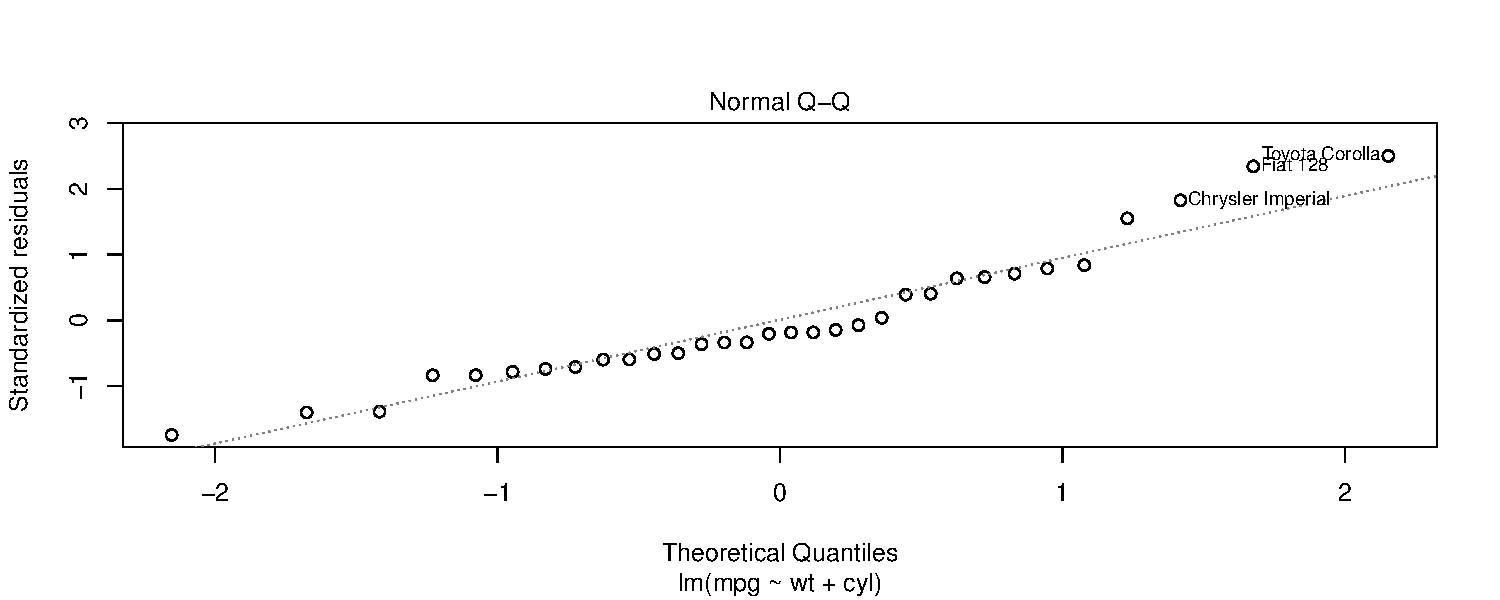
\includegraphics{B3_linreg_files/figure-beamer/unnamed-chunk-24-1.pdf}

\begin{itemize}
\tightlist
\item
  Wenn die Residuen normalverteilt sind, dann sollten sie auf der
  gleichen Linie liegen.
\end{itemize}

\end{frame}

\begin{frame}[fragile]{Regressionsdiagnostik mit Basis-R}

\begin{Shaded}
\begin{Highlighting}[]
\KeywordTok{plot}\NormalTok{(mtcars}\OperatorTok{$}\NormalTok{wt,mtcars}\OperatorTok{$}\NormalTok{mpg)}
\KeywordTok{abline}\NormalTok{(m1)}
\KeywordTok{segments}\NormalTok{(mtcars}\OperatorTok{$}\NormalTok{wt, mtcars}\OperatorTok{$}\NormalTok{mpg, mtcars}\OperatorTok{$}\NormalTok{wt, pre, }\DataTypeTok{col=}\StringTok{"red"}\NormalTok{)}
\end{Highlighting}
\end{Shaded}

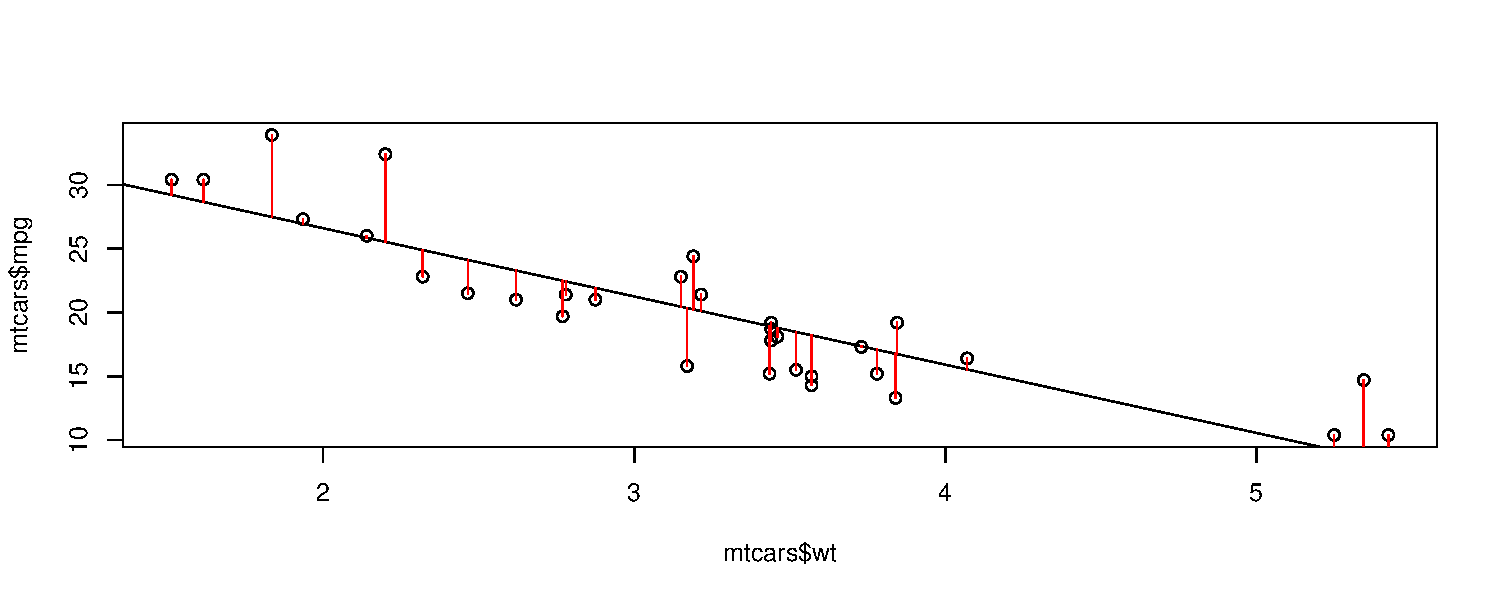
\includegraphics{B3_linreg_files/figure-beamer/unnamed-chunk-25-1.pdf}

\end{frame}

\begin{frame}[fragile]{Das \texttt{visreg}-Paket}

\begin{Shaded}
\begin{Highlighting}[]
\KeywordTok{install.packages}\NormalTok{(}\StringTok{"visreg"}\NormalTok{)}
\end{Highlighting}
\end{Shaded}

\begin{Shaded}
\begin{Highlighting}[]
\KeywordTok{library}\NormalTok{(visreg)}
\end{Highlighting}
\end{Shaded}

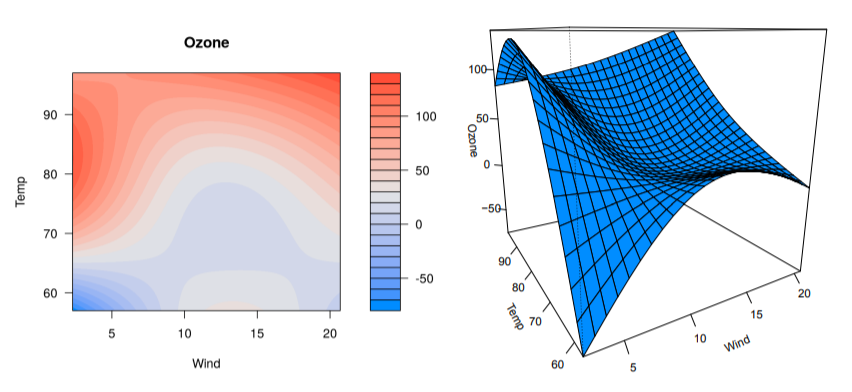
\includegraphics{figure/visreg.PNG}

\end{frame}

\begin{frame}[fragile]{Das \texttt{visreg}-Paket}

\begin{itemize}
\tightlist
\item
  Das Default-Argument für \texttt{type} ist \texttt{conditional}.
\item
  Scatterplot von \texttt{mpg} und \texttt{wt} mit Regressionslinie und
  Konfidenzbändern
\end{itemize}

\begin{Shaded}
\begin{Highlighting}[]
\KeywordTok{visreg}\NormalTok{(m1, }\StringTok{"wt"}\NormalTok{, }\DataTypeTok{type =} \StringTok{"conditional"}\NormalTok{)}
\end{Highlighting}
\end{Shaded}

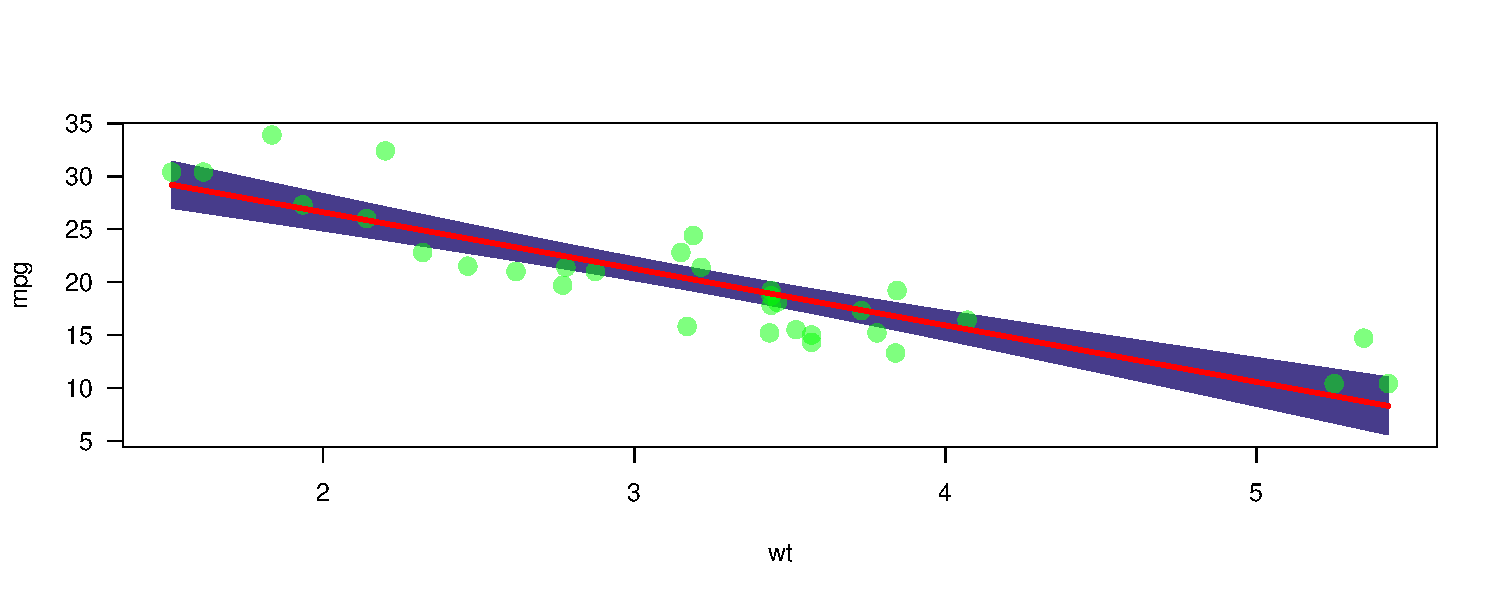
\includegraphics{B3_linreg_files/figure-beamer/unnamed-chunk-30-1.pdf}

\end{frame}

\begin{frame}[fragile]{\href{http://myweb.uiowa.edu/pbreheny/publications/visreg.pdf}{\textbf{Visualisierung
mit \texttt{visreg}}}}

\begin{itemize}
\tightlist
\item
  \href{http://pbreheny.github.io/visreg}{Zweites Argument} -
  Spezifikation der Kovariaten in der Graphik
\item
  Das Diagramm zeigt die Auswirkung auf den erwarteten Wert des
  Regressors, wenn die Variable x von einem Referenzpunkt auf der
  x-Achse wegbewegt wird (bei numerischen Variablen der Mittelwert).
\end{itemize}

\begin{Shaded}
\begin{Highlighting}[]
\KeywordTok{visreg}\NormalTok{(m1, }\StringTok{"wt"}\NormalTok{, }\DataTypeTok{type =} \StringTok{"contrast"}\NormalTok{)}
\end{Highlighting}
\end{Shaded}

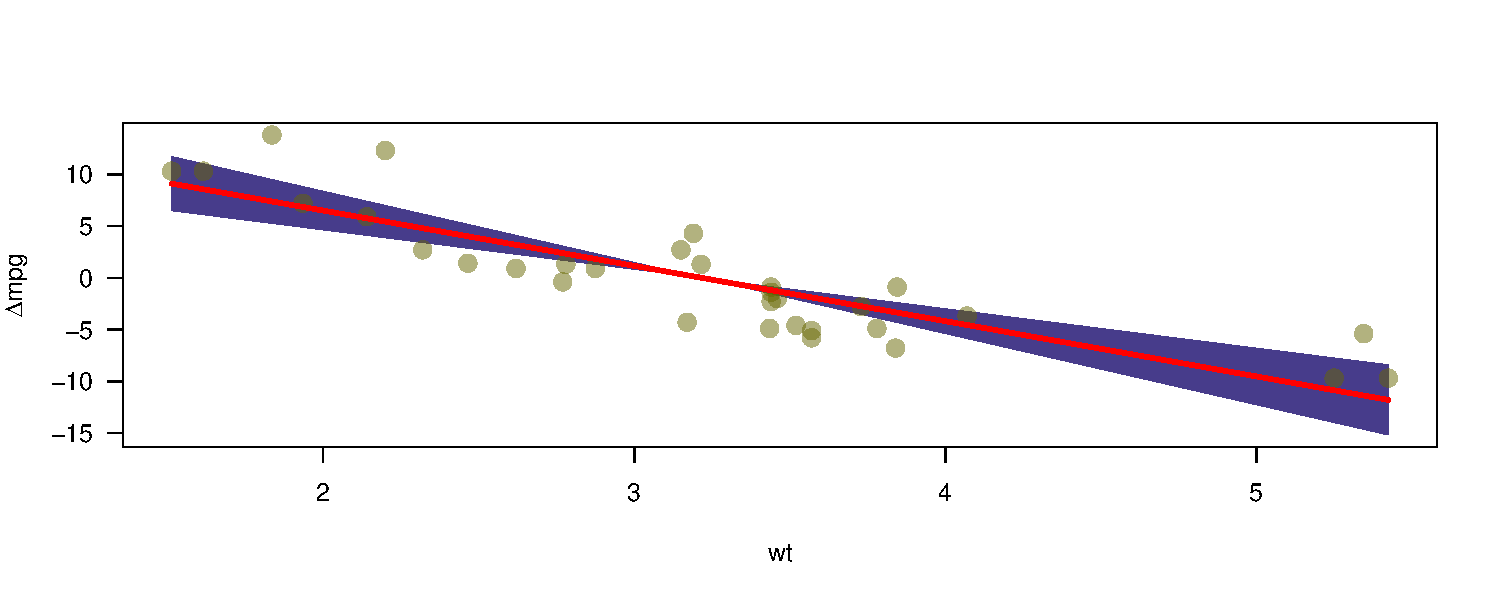
\includegraphics{B3_linreg_files/figure-beamer/unnamed-chunk-32-1.pdf}

\end{frame}

\begin{frame}[fragile]{Regression mit Faktoren}

\begin{itemize}
\tightlist
\item
  Die Effekte von Faktoren können auch mit \texttt{visreg} visualisiert
  werden:
\end{itemize}

\begin{Shaded}
\begin{Highlighting}[]
\NormalTok{mtcars}\OperatorTok{$}\NormalTok{cyl <-}\StringTok{ }\KeywordTok{as.factor}\NormalTok{(mtcars}\OperatorTok{$}\NormalTok{cyl)}
\NormalTok{m4 <-}\StringTok{ }\KeywordTok{lm}\NormalTok{(mpg }\OperatorTok{~}\StringTok{ }\NormalTok{cyl }\OperatorTok{+}\StringTok{ }\NormalTok{wt, }\DataTypeTok{data =}\NormalTok{ mtcars)}
\CommentTok{# summary(m4)}
\end{Highlighting}
\end{Shaded}

\begin{verbatim}
##              Estimate Std. Error   t value     Pr(>|t|)
## (Intercept) 33.990794  1.8877934 18.005569 6.257246e-17
## cyl6        -4.255582  1.3860728 -3.070244 4.717834e-03
## cyl8        -6.070860  1.6522878 -3.674214 9.991893e-04
## wt          -3.205613  0.7538957 -4.252065 2.130435e-04
\end{verbatim}

\end{frame}

\begin{frame}[fragile]{Effekte von Faktoren}

\begin{Shaded}
\begin{Highlighting}[]
\KeywordTok{par}\NormalTok{(}\DataTypeTok{mfrow=}\KeywordTok{c}\NormalTok{(}\DecValTok{1}\NormalTok{,}\DecValTok{2}\NormalTok{))}
\KeywordTok{visreg}\NormalTok{(m4, }\StringTok{"cyl"}\NormalTok{, }\DataTypeTok{type =} \StringTok{"contrast"}\NormalTok{)}
\KeywordTok{visreg}\NormalTok{(m4, }\StringTok{"cyl"}\NormalTok{, }\DataTypeTok{type =} \StringTok{"conditional"}\NormalTok{)}
\end{Highlighting}
\end{Shaded}

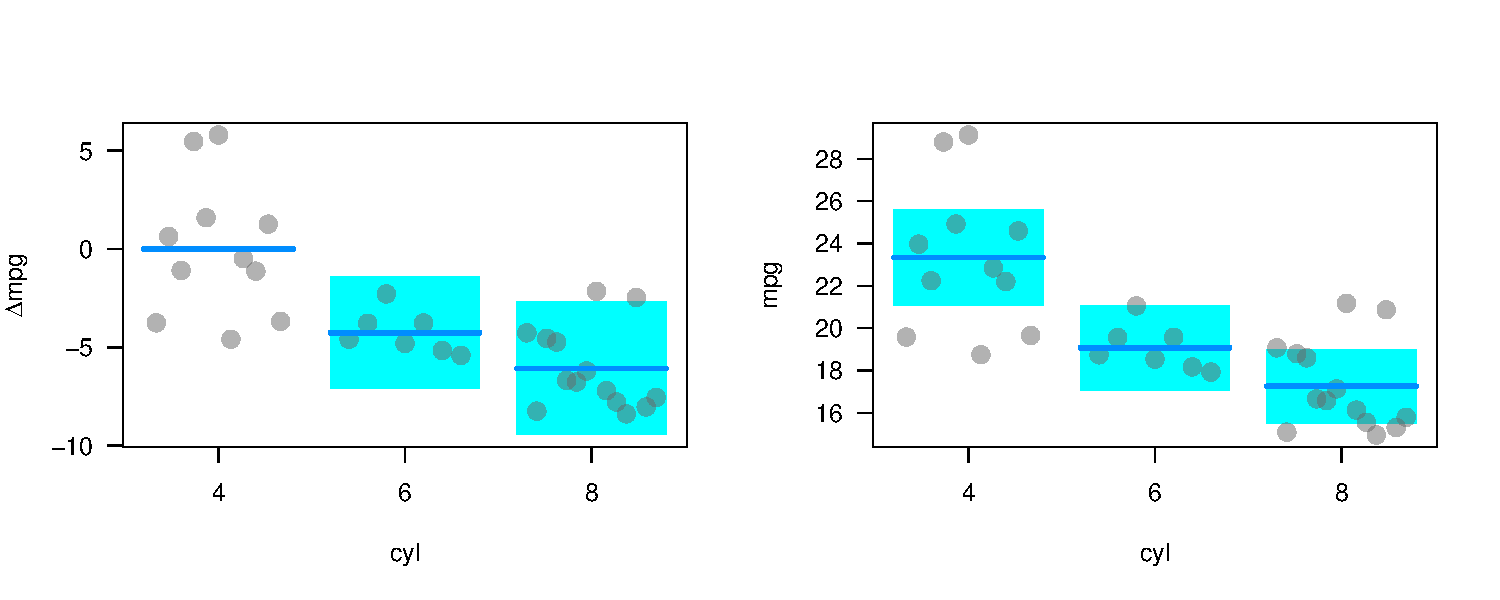
\includegraphics{B3_linreg_files/figure-beamer/unnamed-chunk-36-1.pdf}

\end{frame}

\begin{frame}[fragile]{Das Paket \texttt{visreg} - Interaktionen}

\begin{Shaded}
\begin{Highlighting}[]
\NormalTok{m5 <-}\StringTok{ }\KeywordTok{lm}\NormalTok{(mpg }\OperatorTok{~}\StringTok{ }\NormalTok{cyl}\OperatorTok{*}\NormalTok{wt, }\DataTypeTok{data =}\NormalTok{ mtcars)}
\CommentTok{# summary(m5)}
\end{Highlighting}
\end{Shaded}

\begin{verbatim}
##               Estimate Std. Error    t value     Pr(>|t|)
## (Intercept)  39.571196   3.193940 12.3894599 2.058359e-12
## cyl6        -11.162351   9.355346 -1.1931522 2.435843e-01
## cyl8        -15.703167   4.839464 -3.2448150 3.223216e-03
## wt           -5.647025   1.359498 -4.1537586 3.127578e-04
## cyl6:wt       2.866919   3.117330  0.9196716 3.661987e-01
## cyl8:wt       3.454587   1.627261  2.1229458 4.344037e-02
\end{verbatim}

\end{frame}

\begin{frame}[fragile]{Den Graphikoutput mit \texttt{layout}
kontrollieren}

\begin{Shaded}
\begin{Highlighting}[]
\KeywordTok{visreg}\NormalTok{(m5, }\StringTok{"wt"}\NormalTok{, }\DataTypeTok{by =} \StringTok{"cyl"}\NormalTok{,}\DataTypeTok{layout=}\KeywordTok{c}\NormalTok{(}\DecValTok{3}\NormalTok{,}\DecValTok{1}\NormalTok{))}
\end{Highlighting}
\end{Shaded}

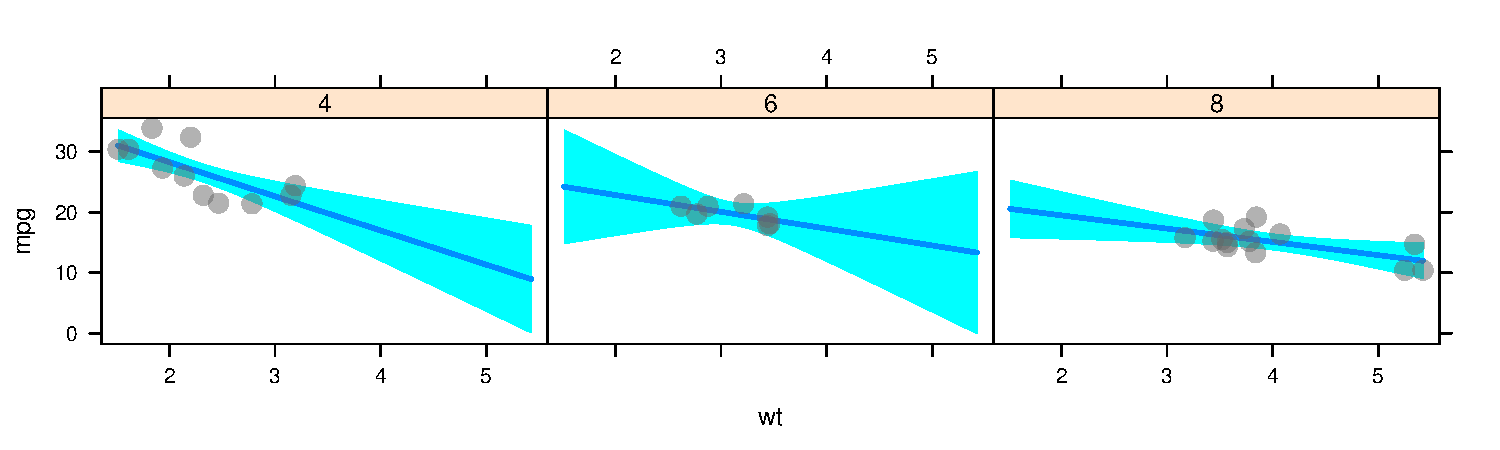
\includegraphics{B3_linreg_files/figure-beamer/unnamed-chunk-40-1.pdf}

\end{frame}

\begin{frame}[fragile]{Das Paket \texttt{visreg} - Interaktionseffekte
übereinander legen}

\begin{Shaded}
\begin{Highlighting}[]
\NormalTok{m6 <-}\StringTok{ }\KeywordTok{lm}\NormalTok{(mpg }\OperatorTok{~}\StringTok{ }\NormalTok{hp }\OperatorTok{+}\StringTok{ }\NormalTok{wt }\OperatorTok{*}\StringTok{ }\NormalTok{cyl, }\DataTypeTok{data =}\NormalTok{ mtcars)}
\end{Highlighting}
\end{Shaded}

\begin{Shaded}
\begin{Highlighting}[]
\KeywordTok{visreg}\NormalTok{(m6, }\StringTok{"wt"}\NormalTok{, }\DataTypeTok{by=}\StringTok{"cyl"}\NormalTok{, }\DataTypeTok{overlay=}\OtherTok{TRUE}\NormalTok{, }\DataTypeTok{partial=}\OtherTok{FALSE}\NormalTok{)}
\end{Highlighting}
\end{Shaded}

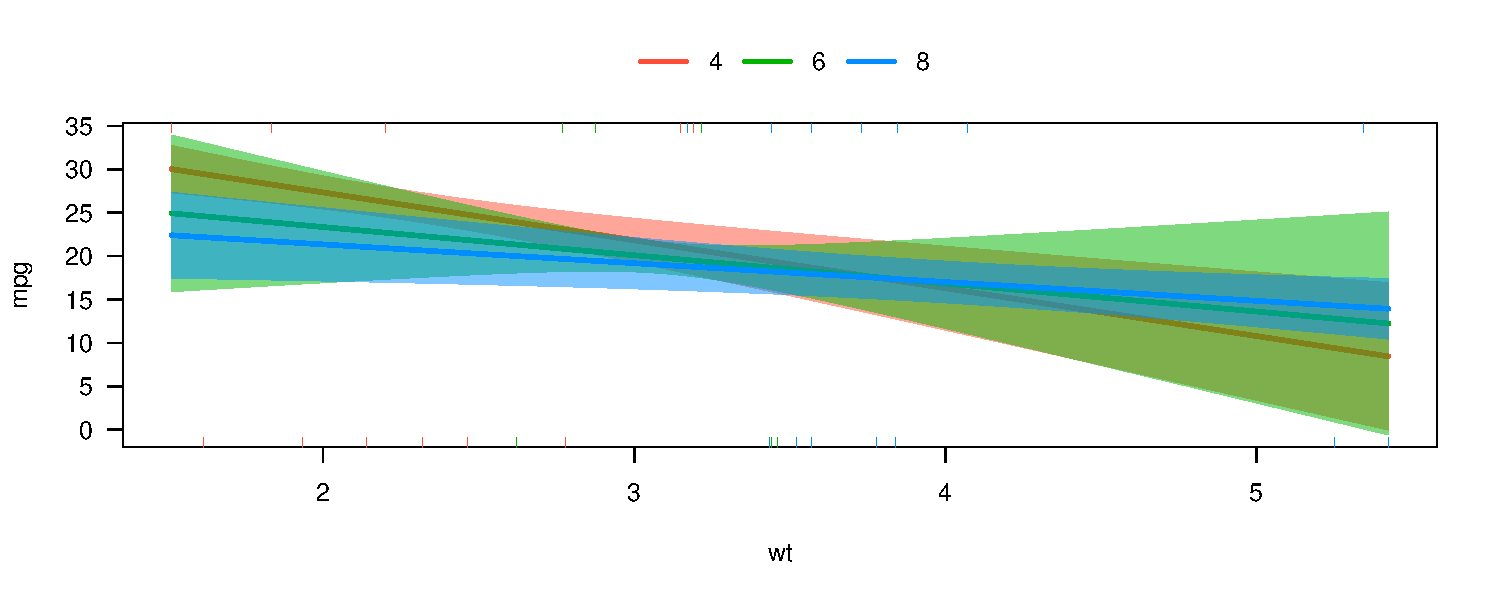
\includegraphics{B3_linreg_files/figure-beamer/unnamed-chunk-42-1.pdf}

\end{frame}

\begin{frame}[fragile]{Das Paket \texttt{visreg} - \texttt{visreg2d}}

\begin{Shaded}
\begin{Highlighting}[]
\KeywordTok{visreg2d}\NormalTok{(m6, }\StringTok{"wt"}\NormalTok{, }\StringTok{"hp"}\NormalTok{, }\DataTypeTok{plot.type =} \StringTok{"image"}\NormalTok{)}
\end{Highlighting}
\end{Shaded}

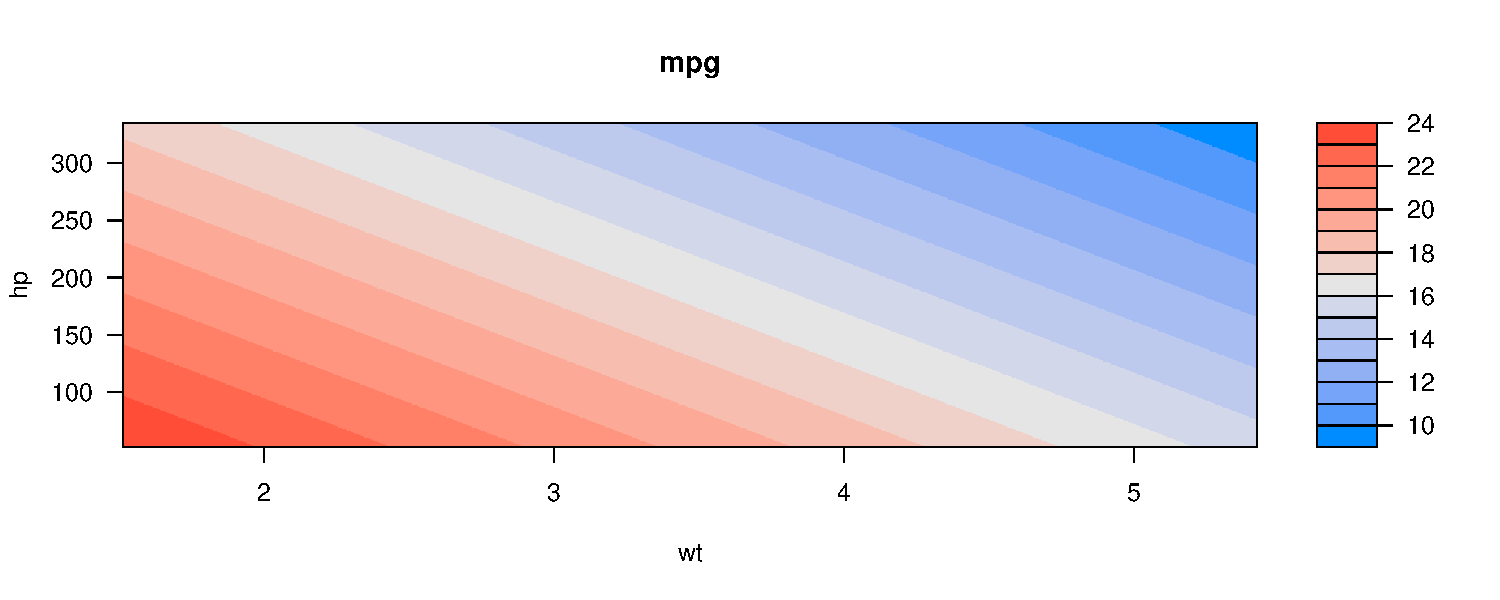
\includegraphics{B3_linreg_files/figure-beamer/unnamed-chunk-43-1.pdf}

\end{frame}

\begin{frame}[fragile]{Das Paket \texttt{visreg} - \texttt{surface}}

\begin{Shaded}
\begin{Highlighting}[]
\KeywordTok{visreg2d}\NormalTok{(m6, }\StringTok{"wt"}\NormalTok{, }\StringTok{"hp"}\NormalTok{, }\DataTypeTok{plot.type =} \StringTok{"persp"}\NormalTok{)}
\end{Highlighting}
\end{Shaded}

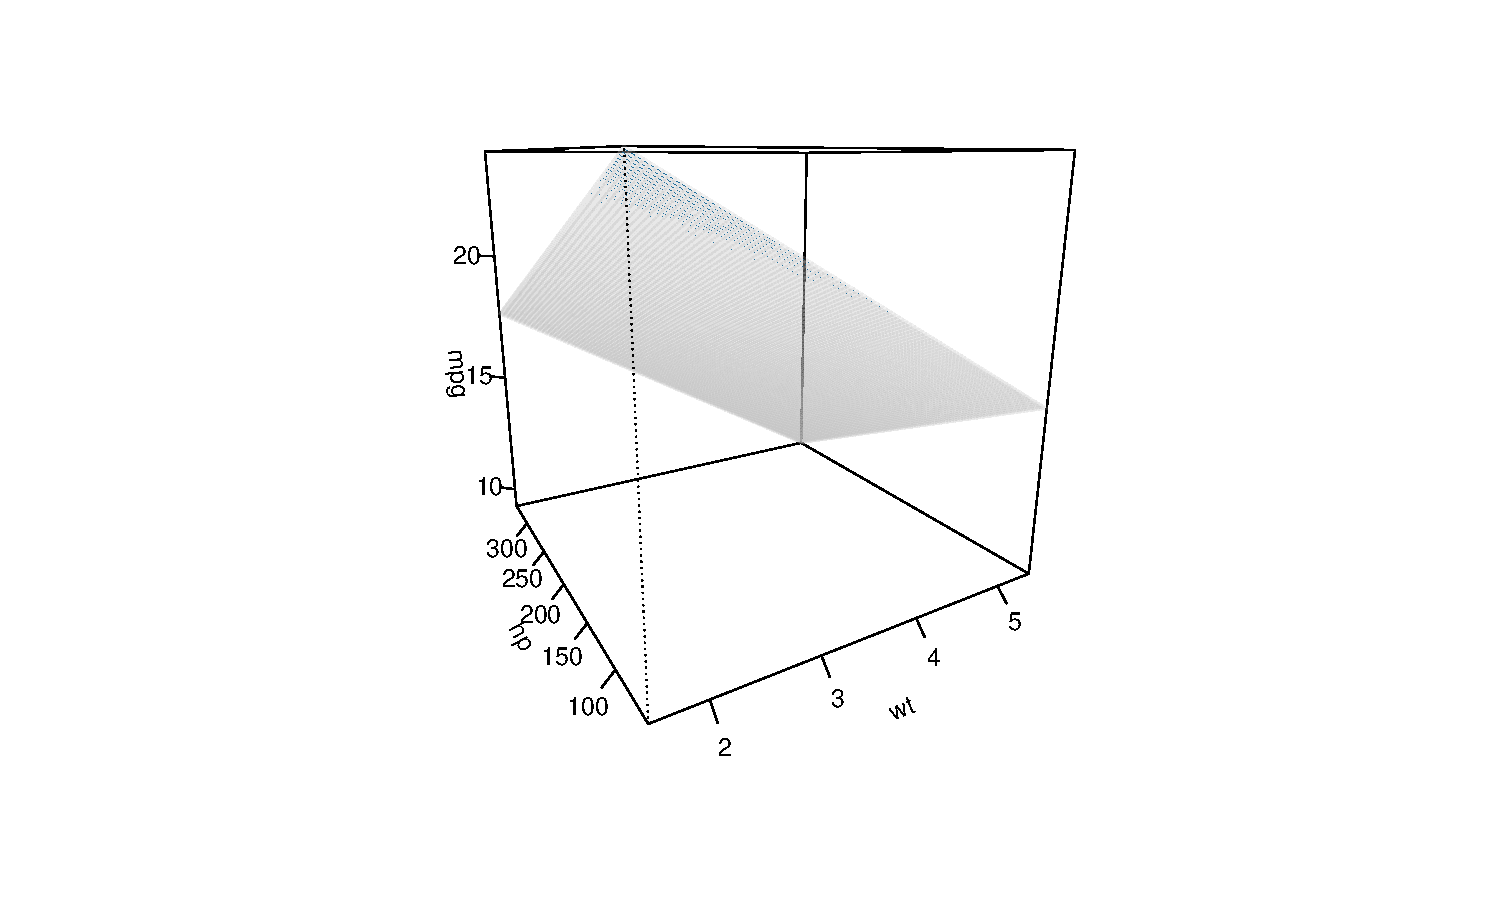
\includegraphics{B3_linreg_files/figure-beamer/unnamed-chunk-44-1.pdf}

\end{frame}

\begin{frame}[fragile]{B3A Aufgabe lineare Regression}

Der Datensatz \texttt{toycars} beschreibt die Route von drei
Spielzeugautos, die Rampen in verschiedenen Winkeln absteigen.

\begin{itemize}
\tightlist
\item
  angle: Rampenwinkel
\item
  distance: Entfernung die von dem Spielzeugauto zurück gelegt wird.
\item
  car: Autotyp (1, 2 or 3)
\end{itemize}

\begin{enumerate}
\def\labelenumi{\alph{enumi})}
\tightlist
\item
  Lese den Datensatz \texttt{toycars} ein und konvertiere die Variable
  \texttt{car} des Datensatzes in einen Faktor (\texttt{as.factor}).
\end{enumerate}

\begin{enumerate}
\def\labelenumi{(\alph{enumi})}
\setcounter{enumi}{1}
\tightlist
\item
  Erstelle drei Box-Plots, in denen die von den Autotypen zurückgelegte
  Strecke visualisiert wird.
\end{enumerate}

\end{frame}

\begin{frame}[fragile]{B3A Aufgabe lineare Regression II}

\begin{enumerate}
\def\labelenumi{(\alph{enumi})}
\setcounter{enumi}{2}
\tightlist
\item
  Schätze für jeden Autotyp getrennt die Parameter des folgenden
  linearen Modell; nutze dafür die Funktion \texttt{lm()}
\end{enumerate}

\[ distance_i= \beta_0 + \beta_1 \cdot angle_i + \epsilon_i\]

\begin{enumerate}
\def\labelenumi{(\alph{enumi})}
\setcounter{enumi}{3}
\tightlist
\item
  Überprüfe die Anpassung des Modells indem Du die drei
  Regressionslinien in den Scatterplot einzeichnest (\texttt{distance}
  gegen \texttt{angle}). Spricht das \[ R^2 \] für eine gute
  Modellanpassung?
\end{enumerate}

\end{frame}

\begin{frame}[fragile]{Einen schönen Output mit dem Paket
\href{https://cran.r-project.org/web/packages/stargazer/vignettes/stargazer.pdf}{\textbf{\texttt{stargazer}}}}

erzeugen

\begin{Shaded}
\begin{Highlighting}[]
\KeywordTok{library}\NormalTok{(stargazer)}
\KeywordTok{stargazer}\NormalTok{(m3, }\DataTypeTok{type=}\StringTok{"html"}\NormalTok{)}
\end{Highlighting}
\end{Shaded}

\begin{block}{Beispiel HTML Outputs:}

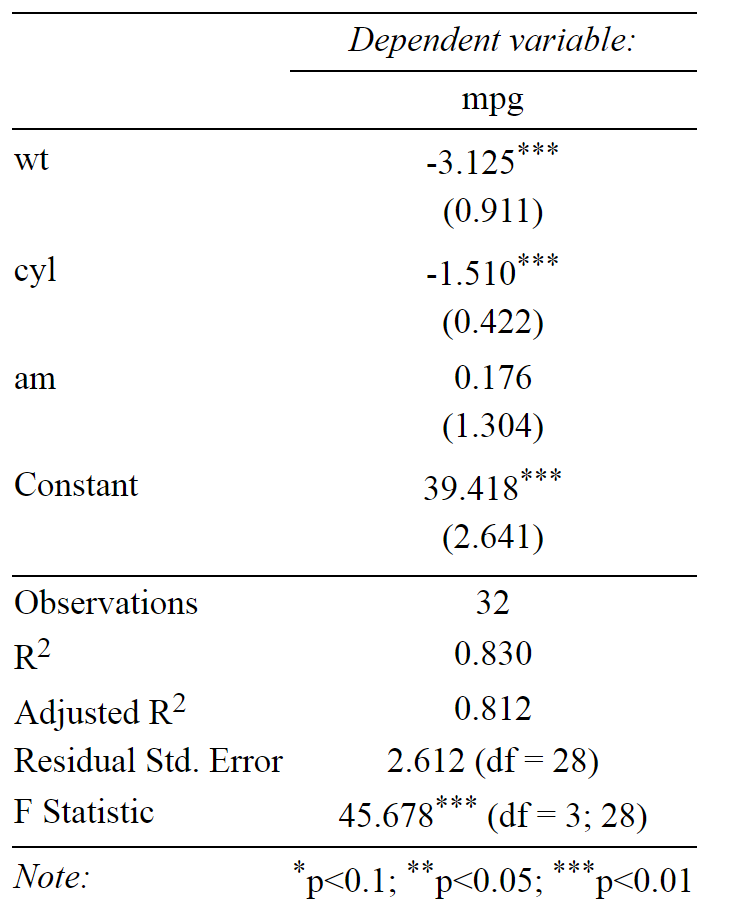
\includegraphics{figure/stargazertabex.PNG}

\end{block}

\end{frame}

\begin{frame}{Shiny App - Diagnostiken für die einfache lineare
Regression}

\url{https://gallery.shinyapps.io/slr_diag/}

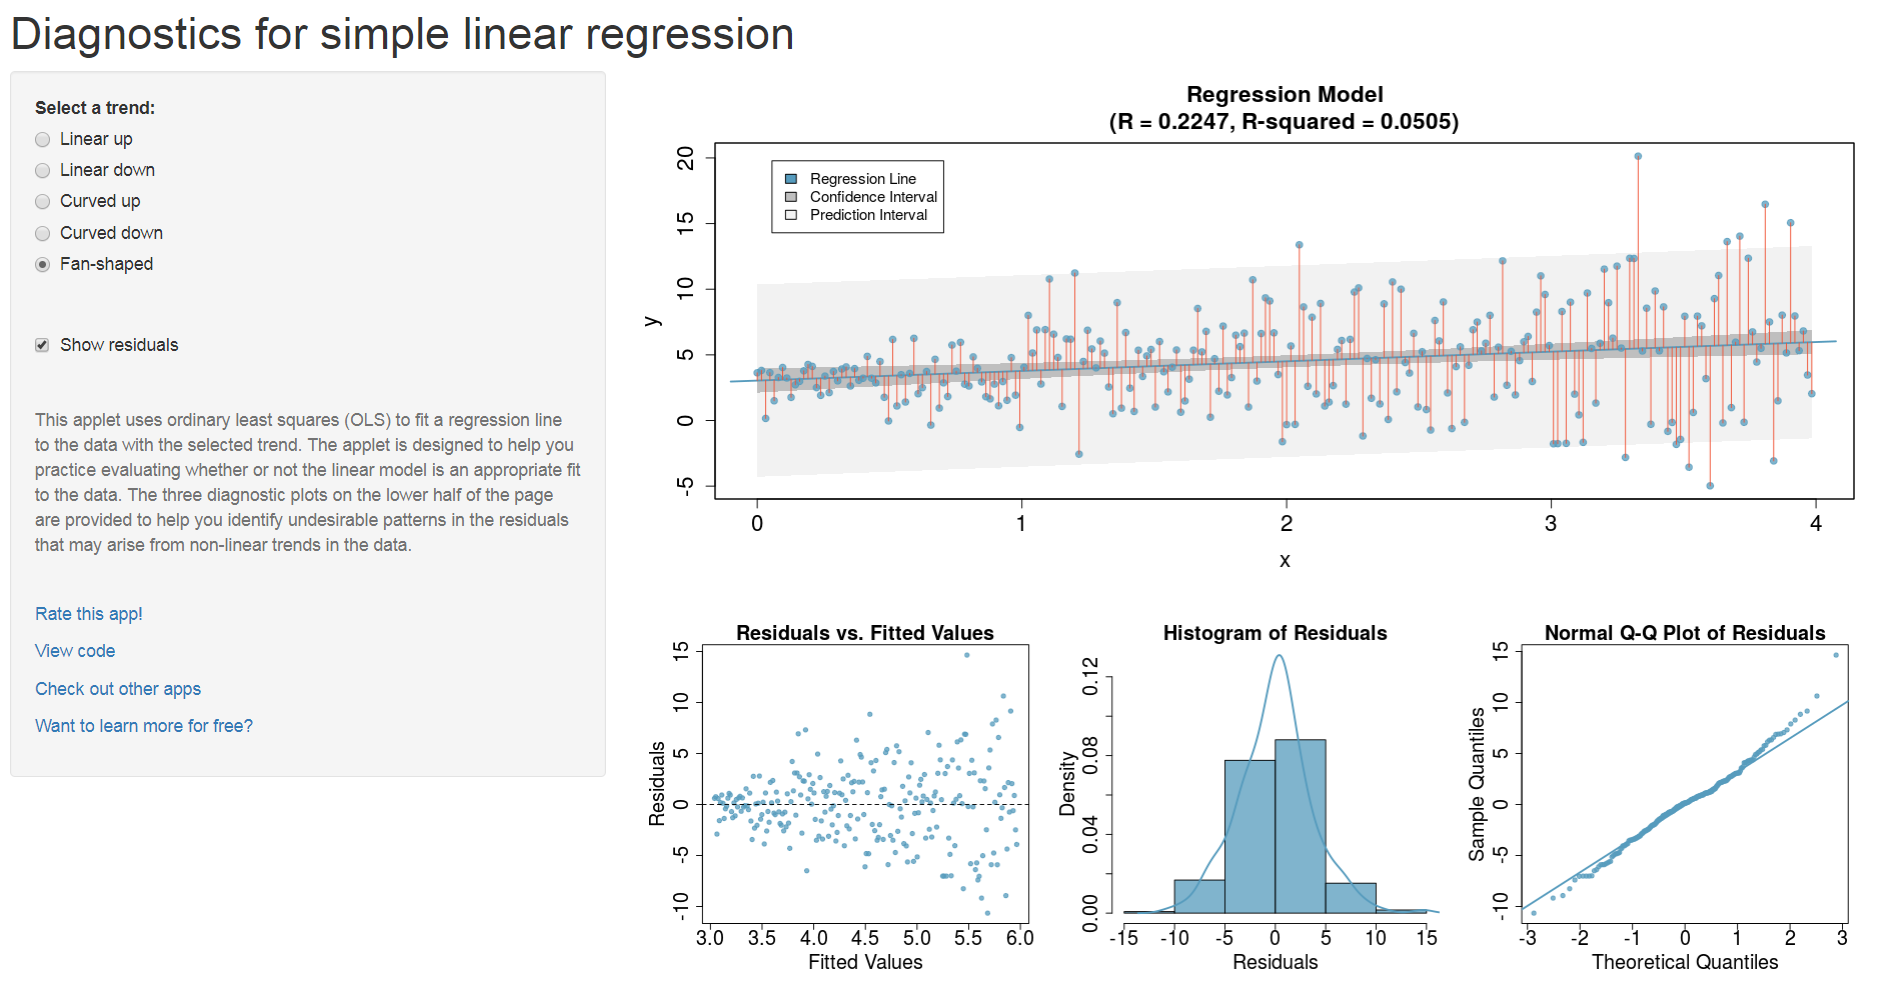
\includegraphics{figure/Diagslr.PNG}

\begin{itemize}
\item
  Shiny App -
  \href{https://gallery.shinyapps.io/simple_regression/}{\textbf{Eine
  einfache lineare Regression}}
\item
  Shiny App -
  \href{figure/https://gallery.shinyapps.io/collinearity/}{\textbf{Multikollinearität
  in multiplen Regressionen testen}}
\end{itemize}

\end{frame}

\begin{frame}[fragile]{Links - lineare Regression}

\begin{itemize}
\item
  Regression -
  \href{http://www.r-bloggers.com/r-tutorial-series-simple-linear-regression/}{\textbf{r-bloggers}}
\item
  Das komplette Buch von
  \href{http://cran.r-project.org/doc/contrib/Faraway-PRA.pdf}{\textbf{Faraway}}-
  sehr intuitiv geschriebenes Buch
\item
  Gute Einführung auf
  \href{http://www.statmethods.net/stats/regression.html}{\textbf{Quick-R}}
\item
  \href{https://www.r-bloggers.com/multiple-regression-part-1/}{\textbf{Multiple
  Regression}}
\item
  \href{https://www.r-bloggers.com/15-types-of-regression-you-should-know/}{\textbf{15
  Arten von Regressionen die man kennen sollte}}
\item
  \href{https://strengejacke.github.io/ggeffects/}{\textbf{\texttt{ggeffects}
  - Erzeuge saubere Datensätze mit marginellen Effekten für `ggplot' aus
  Modell Outputs}}
\end{itemize}

\end{frame}

\end{document}
